{

På samme måde som ovenstående opgave, bruger vi et for-loop til at
simulere 1000 udfald af binomialfordelinger med antalsparameter 8, 20 og
100 og sandsynlighedsparameter $\frac{1}{4}$. Metoden kan findes i
kildekoden og er kaldt \texttt{assignment2\_3\_5()} da de resterende
programmeringsopgaver afhænger af de simuleringer vi kommer frem til.

En simulering laves ved at bruge metoden \texttt{rbinom(n, size, prob)} i
\textbf{R}, hvor $n$ er antallet af observationer, $size$ er
antalsparameteren og $prob$ er sandsynligheden for et gunstigt udfald.

Vi ønsker nu at plotte de observerede værdier for at se dem i forhold til
de teoretiske værdier. Disse kan ses i figur \ref{barplot8_20_100}.
Det ses at de simulerede værdier ligger tæt op ad de teoretiske værdier.
Værdierne er ikke helt ens, men de holder sig i nærheden. Plottene viser
kun de observerede værdier, hvilket kan forklare symmetrien i disse
plots. Ved at sammeligne med figur \ref{binom8_20_100} ses det at der kun
er gjort meget små observationer af de udfald med lille sandsynlighed.
Det mest usædvanlige plot ses i figur \ref{barplot_100}, hvor $x = 24$,
$x = 25$ og $x = 26$ har en lidt større observation end den teoretiske.
En nærmere analyse med et konfidensinterval er ikke blevet foretaget for
at fastslå om de virkelig \emph{er} bemærkelsesværdige. De resterende
observationer viser ikke denne tendens.

\begin{figure}[!h]
    \centering
    \subfloat[$n = 8$ og $p = 0.25$]{
        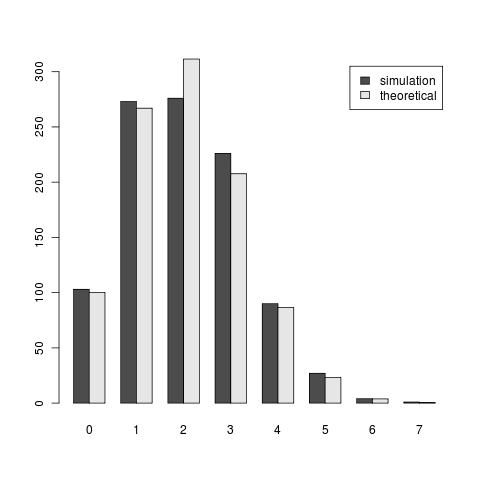
\includegraphics[width=0.5\textwidth]{8_sim-theo_plot_2}
        \label{barplot_8}
    }
    \subfloat[$n = 20$ og $p = 0.25$]
        {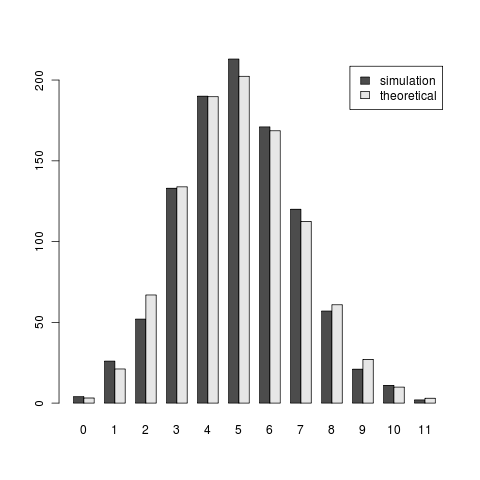
\includegraphics[width=0.5\textwidth]{20_sim-theo_plot_2}
        \label{barplot_20}
    }\\
    \subfloat[$n = 100$ og $p = 0.25$]{
        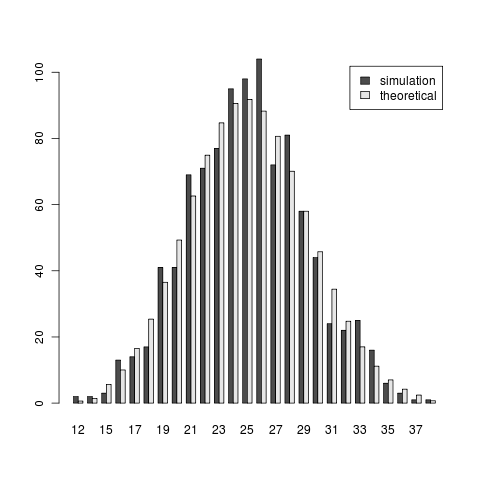
\includegraphics[width=0.5\textwidth]{100_sim-theo_plot_2}
        \label{barplot_100}
    }
    \caption{Barplot af simulerede værdier og de teoretiske værdier.}
    \label{barplot8_20_100}
\end{figure}

}
